\documentclass[sigconf,nonacm]{acmart}
\usepackage{booktabs}
\usepackage{tabularx}
\usepackage{tikz}
\usetikzlibrary{arrows.meta,positioning}
\usepackage{balance}
\usepackage{seqsplit}

\definecolor{hnavy}{HTML}{112B45}
\definecolor{hblue}{HTML}{1E78B4}
\definecolor{hpale}{HTML}{EAF4F8}
\settopmatter{printacmref=false}
\setcopyright{none}
\renewcommand\footnotetextcopyrightpermission[1]{}
\setlength{\textfloatsep}{5pt plus 1pt minus 1pt}
\setlength{\floatsep}{5pt plus 1pt minus 1pt}
\setlength{\intextsep}{5pt plus 1pt minus 1pt}
\setlength{\emergencystretch}{1em}
\renewcommand{\arraystretch}{1.03}

\title{Horizon A1--A6: Runtime Safety with Enforced Singapore Policy Assurance}
\author{Tan Wee Joe}
\affiliation{\institution{University College London}\city{London}\country{United Kingdom}}
\email{tanweejoe@gmail.com}

\begin{document}
\begin{abstract}
Horizon places independent runtime assurance between a vessel's decision AI and its actuators. A1--A5 progressively add probabilistic risk, bounded prediction, barrier filtering, and evidence-conditioned recovery. A6 now enforces a bounded Singapore engineering-policy layer inside the actuator gate: normal A5 commands require policy authorization; withholding triggers checked recovery or explicitly unknown minimum-risk action. Historically, A5 achieved 99.83\% gate acceptance in 12 development branches. New three-seed normal-transit counterfactuals authorized all 72 normal commands under a permissive test policy; a restrictive speed policy admitted zero normal commands and substituted 72 recovery commands. These are synthetic functional experiments, not operational or legal qualification.
\end{abstract}
\keywords{runtime assurance, autonomous vessels, maritime policy, mechanistic interpretability}
\maketitle

\section{Protected system architecture}
The external decision AI may propose heading and speed but cannot command actuators directly. Each proposal is joined with navigation, contacts, uncertainty, platform status, communications, perception, and neural-health evidence. An assurance candidate produces a decision; an exclusive gate then revalidates identity, lineage, freshness, deadlines, actuator limits, and final-command safety. Unknown, stale, late, or unbounded evidence can only preserve or reduce authority. A watchdog retains minimum-risk authority if supervision stops.

\begin{figure}[b]
\centering
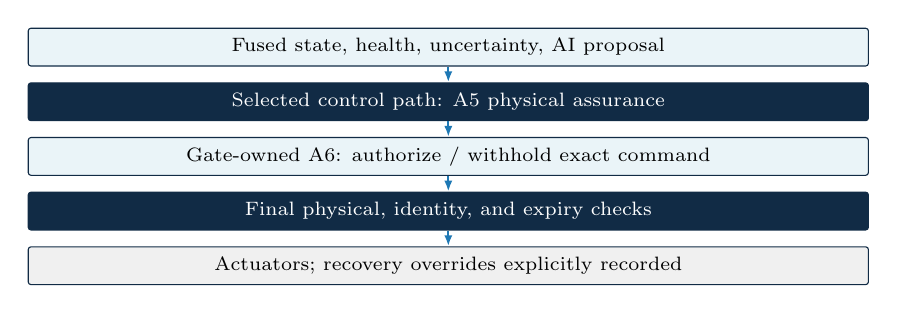
\begin{tikzpicture}[node distance=2mm,every node/.style={font=\scriptsize,align=center},box/.style={draw=hnavy,rounded corners=1pt,minimum width=.88\columnwidth,minimum height=4.8mm,inner sep=1.5pt},arr/.style={-{Latex[length=1.4mm]},hblue,thick}]
\node[box,fill=hpale] (in) {Fused state, health, uncertainty, AI proposal};
\node[box,fill=hnavy,text=white,below=of in] (a5) {Selected control path: A5 physical assurance};
\node[box,fill=hpale,below=of a5] (a6) {Gate-owned A6: authorize / withhold exact command};
\node[box,fill=hnavy,text=white,below=of a6] (gate) {Final physical, identity, and expiry checks};
\node[box,fill=gray!12,below=of gate] (out) {Actuators; recovery overrides explicitly recorded};
\draw[arr] (in)--(a5); \draw[arr] (a5)--(a6); \draw[arr] (a6)--(gate); \draw[arr] (gate)--(out);
\end{tikzpicture}
\caption{Normal actuation requires physical and policy authorization.}
\label{fig:path}
\end{figure}

\section{A1--A6 progression}
All six architectures are deterministic engineering implementations; none uses reinforcement learning. A1--A5 are alternative physical-safety candidates sharing one contract. A6 restricts A5's selected command through the exclusive gate; it does not independently propose maneuvers.

\begin{table}[t]
\centering
\caption{Architectural progression and present disposition.}
\label{tab:architectures}
\scriptsize
\begin{tabularx}{\columnwidth}{@{}lXl@{}}
\toprule
ID & Primary mechanism & Disposition\\
\midrule
A1 & CPA/TCPA thresholds and Simplex switching & baseline\\
A2 & Analytic Gaussian collision-risk approximation & research\\
A3 & Bounded rollout plus complete recovery continuation & retained\\
A4 & Robust barrier correction plus 3DOF validation & retained\\
A5 & Health-conditioned bounds, prediction, A4 filter, recovery & control lead\\
A6 & Gate-enforced Singapore policy checks on exact A5 output & policy layer\\
\bottomrule
\end{tabularx}
\end{table}

\textbf{A1} is transparent and fast, but a threshold result does not establish complete trajectory safety. \textbf{A2} represents uncertainty probabilistically, but its analytic risk score is uncalibrated and is not a hard safety bound. \textbf{A3} adds finite-horizon plant rollout and demands a complete safe continuation before issuance. \textbf{A4} searches the nonlinear vessel map for a barrier-compatible correction and validates the result with a full rollout. \textbf{A5} makes that path evidence-aware: healthy evidence retains nominal bounds and a 6\,m/s cap; degraded required evidence expands bounds by 1.5 and caps speed at 3\,m/s; invalid required evidence forces fallback. It attempts predictive recoverability, invokes A4 when needed, and falls back on incomplete, infeasible, or late results.

\textbf{A6} evaluates bounded engineering proxies for Rules 5--8 and 13--17. The development profile is a 12\,m, 40\,GT Singapore government USV under remote supervision in daylight and clear visibility. Source artifacts are hash-checked at load; fresh evidence binds the snapshot and command. Actual course/speed changes override adapter action claims. Unknown, unsupported, late or unsatisfied evidence withholds authority. Normal dispatch must precede policy, evidence and cycle expiry. Emergency recovery remains available and is labelled as a policy override. MASS design references and the broader maritime-policy context motivate the bounded model~\cite{imo-colreg,imo-mass,rsn-usv}; these engineering predicates do not establish statutory compliance.

\section{A1--A5 comparative results}
The initial development matrix contained 12 paired identities: four scenarios, three seeds, and five candidates per identity, for 60 branches. Scenarios covered recoverable crossing, dense traffic, vessel degradation, and initially unrecoverable encounters. Timing was idealized except for 20\,ms candidate and gate service, so the study compares architecture behaviour rather than production latency.

\begin{table}[t]
\centering
\caption{A1--A5 development study; 12 branches per candidate.}
\label{tab:controller}
\scriptsize
\begin{tabular}{@{}lrrrr@{}}
\toprule
 & Gate & Deadline & Recoverable & Unsafe/stale\\
ID & accepted & misses & collisions & accepted\\
\midrule
A1 & 8.87\% & 0 & 0 & 0\\
A2 & 8.73\% & 1 & 0 & 0\\
A3 & 99.66\% & 6 & 0 & 0\\
A4 & 99.44\% & 10 & 0 & 0\\
\textbf{A5} & \textbf{99.83\%} & \textbf{3} & \textbf{0} & \textbf{0}\\
\bottomrule
\end{tabular}
\end{table}

None of the 45 declared-recoverable branches collided; all 15 deliberately unrecoverable branches collided. No unsafe or stale result was accepted. A1 and A2 often passed proposals the independent predictive gate rejected, producing acceptance below 9\%. A3--A5 actively selected recovery or minimum-risk commands and exceeded 99.4\% acceptance. A5 had the highest acceptance and fewer deadline misses than A3 or A4, so it became the physical-control lead. These small, development-set results do not prove statistical superiority or operational safety.

\section{A6 shadow baseline and enforcement}
\begin{sloppypar}
The earlier shadow run reused the 12 historical A5 episode identities, hashes, policies and 30-second horizon. It observed 1,788 decisions: 888 recovery, 885 minimum-risk and 15 invalid. All withheld policy support; median A6 latency was 0.178\,ms. This established conservative shadow behavior, but could not demonstrate enforcement on permissive commands.
\end{sloppypar}

\begin{table}[t]
\centering
\caption{New normal-transit counterfactuals: 3 seeds, 5 s each.}
\label{tab:a6}
\scriptsize
\begin{tabularx}{\columnwidth}{@{}Xr@{}}
\toprule
Measure & Result\\
\midrule
A5-only normal commands accepted & 72\\
A6 permissive: authorized / normal accepted & 72 / 72\\
A6 speed veto: normal / recovery accepted & 0 / 72\\
A6 speed veto: initial vetoes / latched recoveries & 3 / 69\\
Command-trace mismatches / collisions & 0 / 0\\
\bottomrule
\end{tabularx}
\end{table}

The enforcement experiment compares A5 alone with two synthetic policy bundles on the same normal-transit seeds. The 6\,m/s test cap permits normal commands; the 1\,m/s cap vetoes the first command in each seed and latches recovery thereafter. Each arm also records 69 watchdog commands and 72 command-expiry events. The local-acceptance timing model has zero simulated gate service; measured wall work is separate. These results establish functional authorization and veto behavior, not timing readiness or uninterrupted autonomy. The implementation also corrects recovery priming's simulated-to-host deadline mapping.

The original 12-episode, 30-second matrix was also rerun with enforcement: 1,770 gate acceptances and 18 deadline rejections, comprising 885 recovery, 885 minimum-risk and 18 invalid decisions. No normal command reached policy evaluation; these actions were explicit emergency overrides. Trace mismatches were zero; the three initially-unrecoverable episodes remained unsafe. Host-sensitive deadline counts are revision/run-specific.

\section{Why the A5+A6 composition was selected}
\textbf{A5 remains the physical-control lead}: it combines evidence-conditioned conservatism, recovery validation and favorable historical acceptance. \textbf{A6 is chosen as mandatory policy authorization}: the new counterfactuals show that changing policy changes which physically permissible commands reach the plant. Its assessments bind the complete input, decision, evidence and versioned bundle. This closes the previous observation-only gap while retaining physical revalidation and explicit emergency authority.

Restricted visibility, channel/TSS navigation, unknown vessel classes and broader profiles withhold authorization. Weapons, targeting, classified doctrine and ROE remain excluded. This release vetoes A5's single selected command; it does not search alternative policy-compliant maneuvers. Recorded operational sources, live evidence integration, legal review and target-platform timing remain qualification work.

\section{Neural-health input and verdict}
H5 monitors WaSR-T's temporal-fusion representation with a hash-pinned sparse feature. Its selected development feature beat random-direction and equal-norm causal controls in all 18 trials. An optional simulation-warning mode can reduce the AI's proposed speed; operational calibration remains unqualified. H5 cannot prove obstacle-free water or increase A5/A6 authority.

The product now defaults to \emph{A5 with enforced A6 authorization}. Without configured recorded sources and fresh policy evidence, normal autonomy is withheld. Recovery overrides are visible in gate telemetry and receipts. The delivered software enforces the bounded policy model; the evidence does not qualify autonomous vessel deployment or full maritime-law compliance.

\paragraph{Reproducibility.}
\begin{sloppypar}
Counterfactuals: \path{scripts/benchmark_a6_enforcement.py}. Result: \path{horizon-runs/development/a6-enforcement-counterfactual-20260925-v5/summary.json}. SHA-256: \texttt{\seqsplit{0f63c151344bf6f576257d38efc0302c511f0df127987d9f95223dbbf32543f1}}. Original scenario matrix: \path{experiment/manifests/a6-a32-enforcement-development.json}.
\end{sloppypar}

\balance
\begin{thebibliography}{3}
\bibitem{imo-colreg} International Maritime Organization. \emph{Convention on the International Regulations for Preventing Collisions at Sea (COLREGs)}. \url{https://www.imo.org/en/about/conventions/pages/colreg.aspx}.
\bibitem{imo-mass} International Maritime Organization. \emph{Autonomous shipping}. \url{https://www.imo.org/en/mediacentre/hottopics/pages/autonomous-shipping.aspx}.
\bibitem{rsn-usv} Ministry of Defence Singapore. \emph{Republic of Singapore Navy's Maritime Security Unmanned Surface Vessels Commence Operational Patrols}, 2025. \url{https://www.mindef.gov.sg/news-and-events/latest-releases/04feb25_fs/}.
\end{thebibliography}
\end{document}
